% this file is called up by thesis.tex
% content in this file will be fed into the main document

%: ----------------------- name of chapter  -------------------------
\chapter{Taxonomy and Model of Inter-Thread Communication} % top level followed by section, subsection
\label{chapterModel}

%: ----------------------- paths to graphics ------------------------

% change according to folder and file names
\ifpdf
    \graphicspath{{X/figures/PNG/}{X/figures/PDF/}{X/figures/}}
\else
    \graphicspath{{X/figures/EPS/}{X/figures/}}
\fi

%: ----------------------- contents from here ------------------------

This chapter describes a developed mathematical model of the involvement of cache in inter-thread data transfer. Creation of the exact model of what is expected when data is shared between threads that reside on different parts of the processor is a complex undertaking. Processor hardware is updated rapidly and each new generation of CPUs incorporates unseen before technologies that require more complex models that can describe the inter-thread communication. Such model is created to predict the impact of scheduling of the receiving thread for any CPU, it allows to generalise the proposed solution. It helps to develop the experiments that allow to characterise the performance of the data transfer through different levels of cache and main memory. In order to measure the impact of scheduling, the model is required as well. A number of resources of existing models of the cache are discussed in this chapter. Analysis of cache of inter-thread communication leads to a taxonomy shown in the next section. 

\section{Taxonomy of Inter-Thread Communication}
\label{taxonomy}

Multi-core systems handle usage of cache in multi-threaded programmes differently. Cache in most modern-day processors is organised in the following way: \textit{Level 1} (L1) and \textit{Level 2} (L2) data and instruction caches are private for each core and \textit{Level 3} (L3) cache is shared. Besides the mentioned in section \ref{cacheLit} Intel 64 architecture, such hierarchy is also commonly used in products of other manufacture, for example, IBM's POWER7 \cite{IBM2010} and AMD's Opteron \cite{Conway2011} chips that are utilised in servers and workstations. Additionally, in this type of architecture, private for each core levels of cache are inaccessible by private levels of cache associated with other cores. The private cores are each connected to the shared cache (normally L3) via the shared data bus. Providing external access to processors' cache memory is problematic, since caches from different levels have no direct physical connections between them. If one core needs to access data that is stored in another core's cache, the only way to receive required information is through the system bus.

In case of a processor where each core has a private L1 cache and shared between cores of the same CPU L2 caches, there can be three main patterns of thread communication. Refer to Figure \ref{Threads_cpu_diagram} for a diagram that outlines these patterns. It is assumed that no thread scheduling takes place. 

\begin{figure}[ht!]
\centering
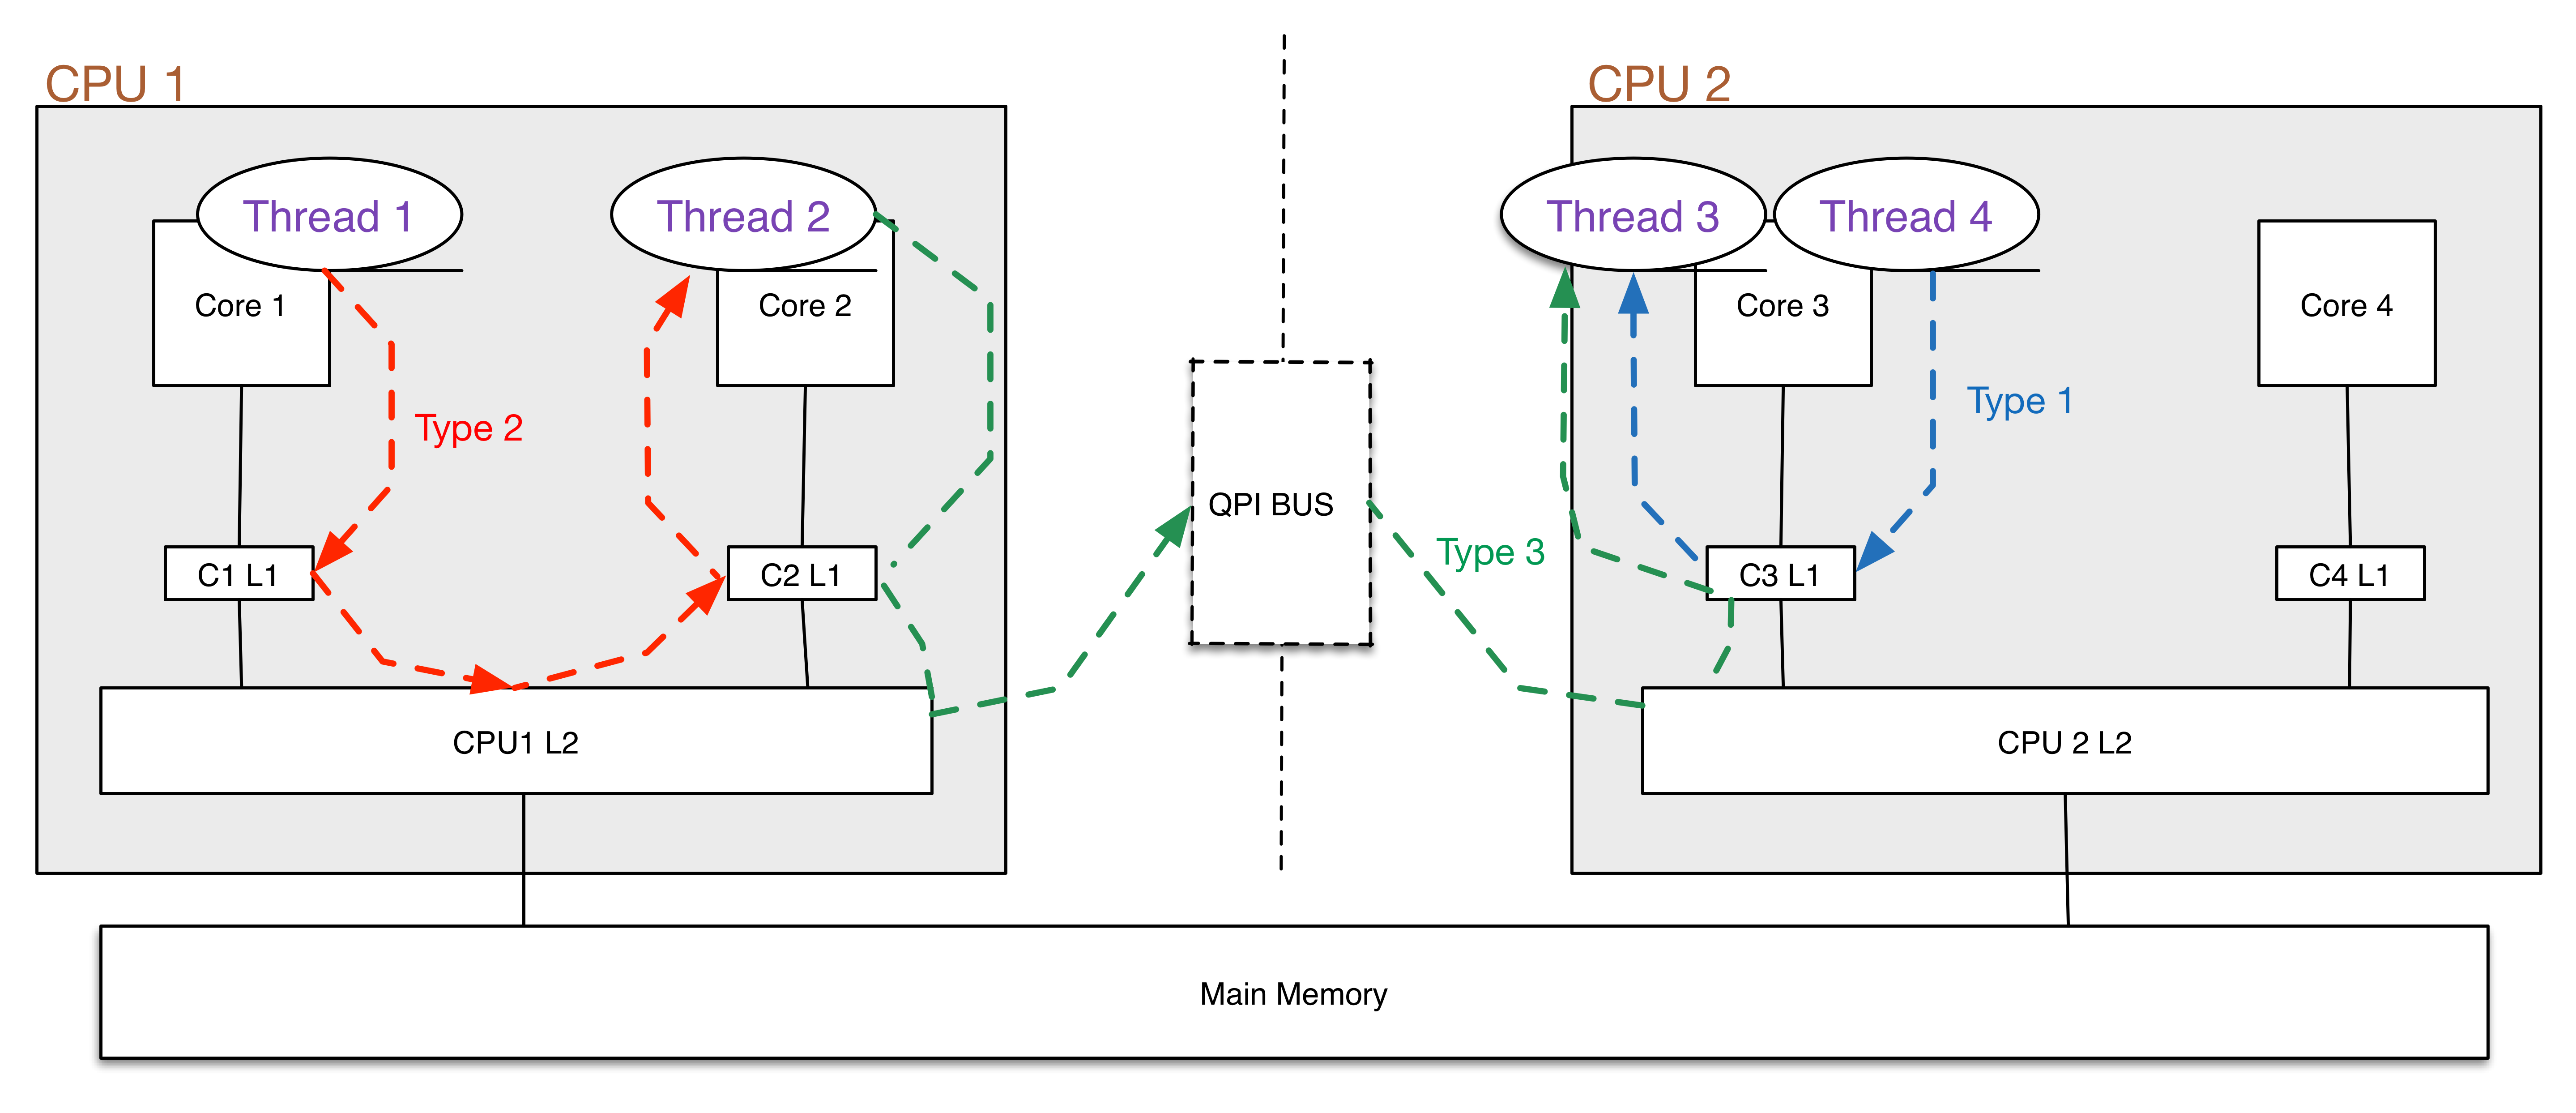
\includegraphics[width=145mm]{3/Threads_cpu_diagram.png}
\caption{Communication between threads in a multi-core environment}
\label{Threads_cpu_diagram}
\end{figure}

The following list presents the taxonomy of inter-thread exchange of data that defines three types of communication:

\begin{description}
  \item[Type 1] The simplest case that is associated with the least amount of overhead caused by moving data between threads (Thread 3 and Thread 4) is communication between two threads that reside on \textit{the same CPU, same core}. The blue line on the figure represents this scenario.
  \item[Type 2] Communication takes place between two threads that are executed by \textit{the same CPU, but they reside on different cores}; this type of communication is more expensive\footnote{\textit{expensive} -- takes a significant amount of time to execute.} computation-wise (compared to Type 1) because different L1 and L2 caches are utilised when the threads use shared data. The red line on the diagram shows an example of communication of this type. 
  \item[Type 3] The most complicated case involves all three levels of cache. In this case data is shared between threads that reside \textit{on different chips}. An inter-chip bus has to be used. The green line points to an example of communication of this type
\end{description}

The cost of inter-thread communication depends on the nature of the task that needs to be performed (i.e. amount of I/O, amount of data used etc.), the environment (primarily the choice of the processor) and a number of other attributes of the system used. Usage of a scheduler that is cache-aware may greatly improve the efficiency of cache in multi-core systems and hence the overall performance. One may find a few schedulers that are aimed at multi-threaded programmes \cite{Zhuravlev2012,Liaskovitis2006,Chen2007}. Two systems that claim to support cache-aware scheduling are Parallels Depth First (PDF)\cite{Blelloch1999} and Work Stealing (WS)\cite{Blumofe1994}. Both of them were built in 1990s, in the pre-multichip era.

\section{Model of Inter-Thread Communication}
\label{modelsection}

A number of resources discuss existing models of the cache \cite{ChenDing,Agarwal1989,Song2007}. A model suggested by the authors of \cite{ChenDing} was thoughtfully tested by a number of benchmarks and the findings presented in the paper were used as motivation for creation of the proposed in this section model. However, the referred model does not take into account exchange of data on the main memory level. Similarly, \cite{Song2007} discusses the L2 cache only. Work published in \cite{Agarwal1989} was conducted in the end of 1980s, and the proposed in that paper model proves to be too abstract, when applied to current computer architectures. A few papers discuss the implications of conducting simulations \cite{Heidelberger1990,Archibald1986,Zhao2011} rather than describing the behaviour of cache by means of mathematical modelling. The mathematical description of the inter-thread communication provides a much more solid grounding for further research. Creation of such model is undertaken within the scope of this study, because it allows to predict the impact of scheduling decisions for any CPU that the model can be applied for.

The proposed model describes communication between two threads that reside on a system that has three levels of cache. The Level 1 caches are private for each core, the Level 2 caches are private for each chip. The Level 3 caches are private for each chip, but, in case of most modern-day processors, they are connected by a bus, which, effectively, unites them and combines the caches into one shared across the whole processor entity. Such model is later tested by performing experiments on the real hardware.

The activity being analysed in this model is where the first thread Th1 writes data into caches, making the thread the sending end, and the second thread Th2 reads data, which makes it the receiving end. Time, which needs to be spent on writing data to a buffer in one thread, and then reading it out of that buffer in another thread, is modelled. The interaction between the size of the buffer and the cache size(s) is modelled. This scenario is an example of a simplified version of a typical ``client--server" application. Such programmes can often be seen in the telecommunication industry, where large quantities of data are exchanged between clients and servers. Analysis of such simplified case can be a base for further work that involves more complicated programmes.

There is one variable in the model: the size of data that is shared between two threads $n$. The quantum of stored data is one cache line (typically 64 or 128 bytes). Depending on the size of used data, information is stored in a cache (-s) of a particular level; i.e. if data fits into Level 1 cache, it is stored there, if not, it is cached in the next level of cache -- Level 2 cache.

The latency of using shared between two threads data (Thread 1 writes data into a cache or main memory and Thread 2 reads data from the cache or main memory) $d_{comm}$ can be described by an equation \eqref{eq:model1}:

\begin{equation}\label{eq:model1}
d_{comm} = d_{write} + Control + d_{read}
\end{equation}

, where the cost of writing data into the cache $d_{write}$ is described by equation \eqref{eq:model2}:

\begin{equation}\label{eq:model2}
d_{write} = \begin{cases}d_{WriteL1}= n/ns * lat_{WriteL1} & n \leq l_{L1}\\d_{WriteL2} = n/cls * lat_{WriteL2} + l1w & l_{L1} < n \leq l_{L2}\\d_{WriteL3} = n/cls * lat_{WriteMem} + l1w & l_{L2} < n \leq l_{L3}\\d_{WriteMem} = n/cls * lat_{WriteMem} + l1w & n > l_{L3}\end{cases}
\end{equation}

, where $l_{L1}$, $l_{L2}$, $l_{L3}$ indicate sizes of Level 1, Level 2, and Level 3 caches respectively. $ns$ points to the size of one word of data that is written in cache, e.g. 4 bytes for a case of using \textit{long} on most systems. As described in section \ref{cacheLit}, the minimum amount of data that can be fetched from caches is a cache line; in this model, $cls$ is the size of one cache line. $l1w$ indicates the cost of writing the amount of memory that can fit into Level 1 cache. In most cases this number is small and can be neglected. The model assumes that direct mapped caches are used.

\begin{equation}\label{eq:model20}
l1w = (n/ns - n/cls) *  lat_{WriteL1}
\end{equation}

Figure \ref{cacheline} gives an example of writing and reading one cache line, when the access is initiated from main memory. In this case the size of a cache line is 64 bytes and long words (4 bytes each) are written/read. The first write/read is very expensive because all levels of memory are used and its latency is equal to the latency of the level in memory, from which the operation was initiated. All subsequent actions are performed solemnly on the Level 1 cache and the latency of such operations equals to the latency of Level 1 cache. $l1w$ can be expressed by equation \ref{eq:model20}. The caches are assumed to be fully associative for simplicity, i.e. n-associativity of cache is ignored. It is also assumed that neither pipelining no simultaneous execution of multiple instructions are implemented.

\begin{figure}[ht!]
\centering
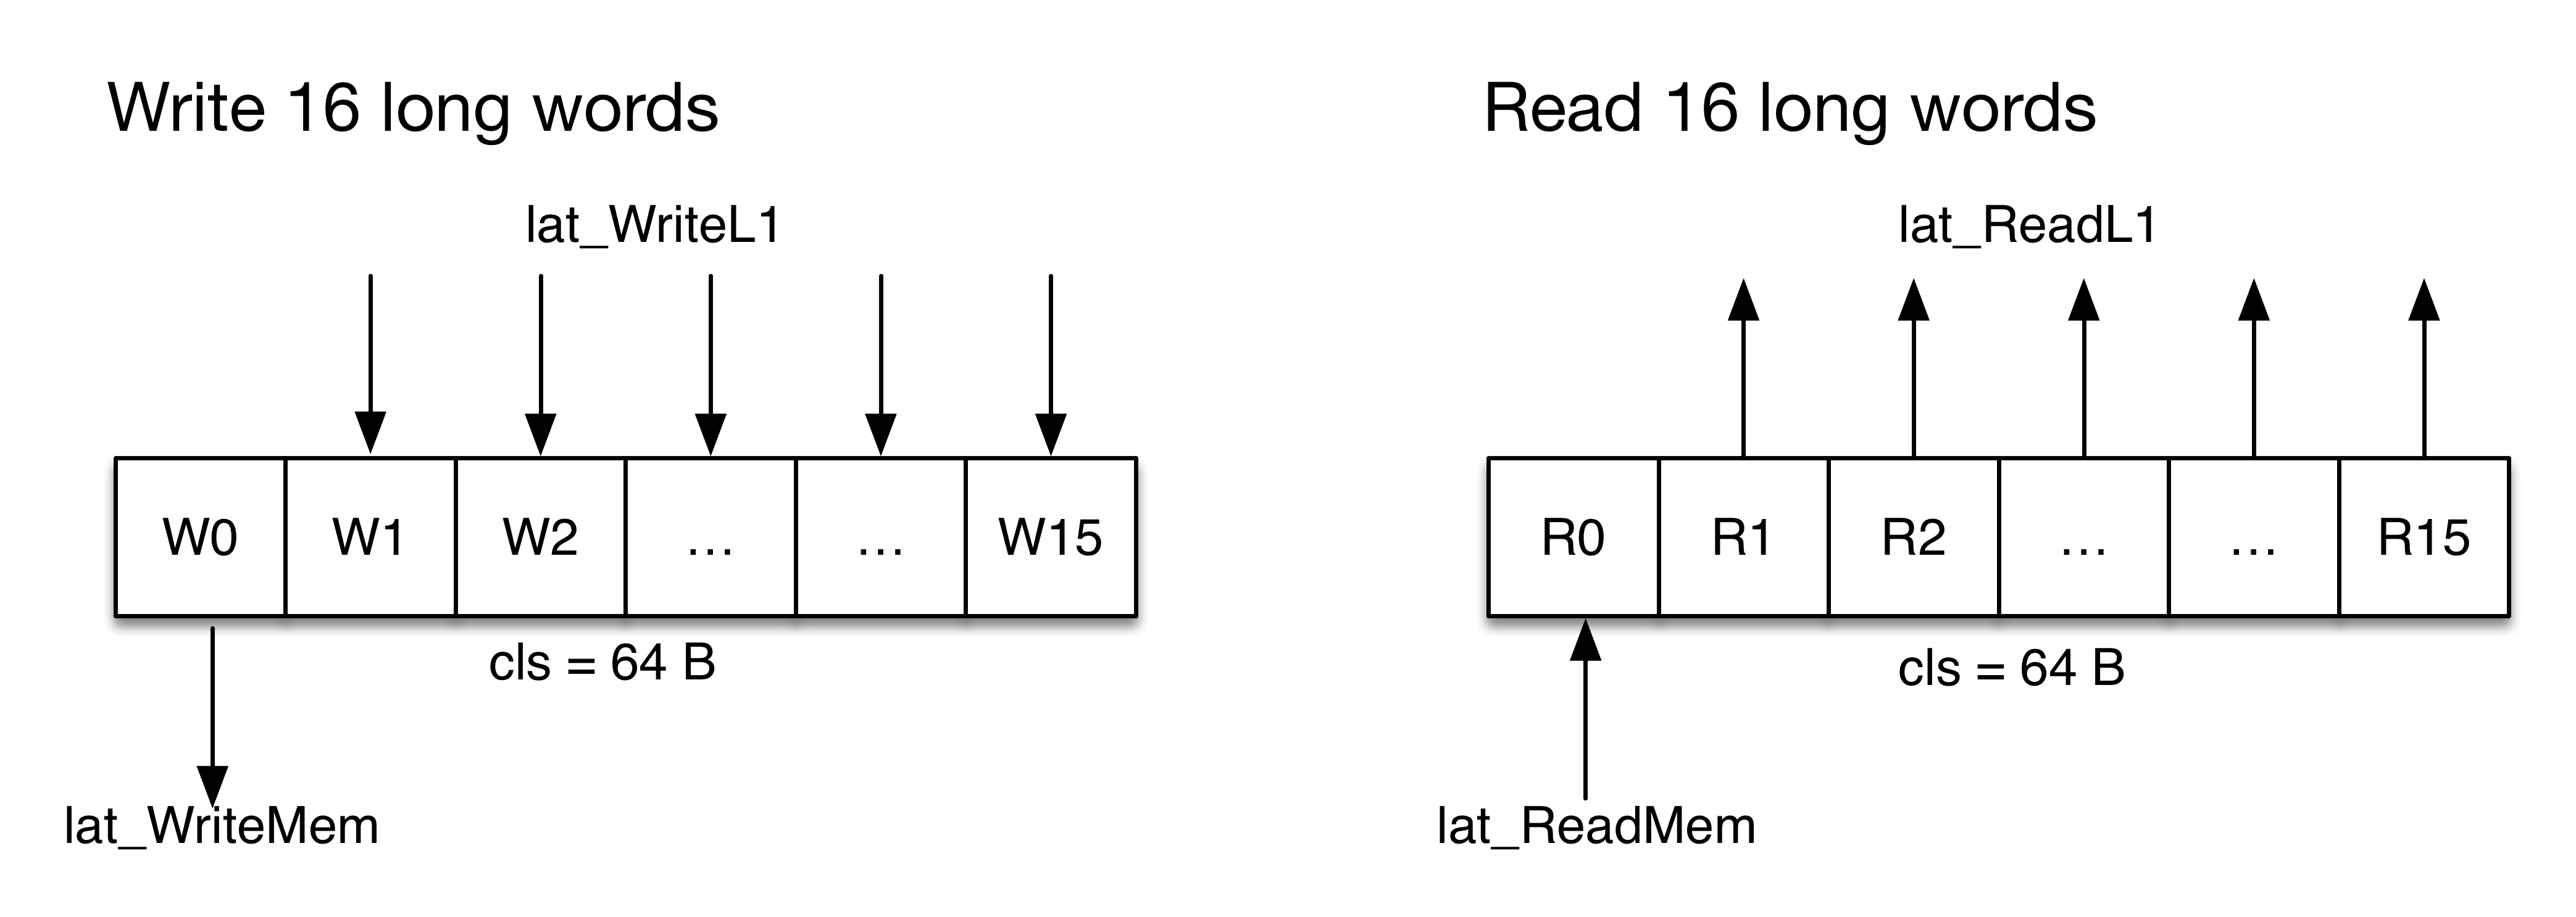
\includegraphics[width=145mm]{3/cacheline.png}
\caption{Writing and reading a cache line in a Write-back cache}
\label{cacheline}
\end{figure}

Utilisation of threads implies that there will also be overhead caused by the control element. In the situation of having two POSIX-threads\footnote{\textit{POSIX-threds} is a POSIX standard for threads. This technology is utilised to control threads in a multi-threaded environment in the project.} working with shared data, the overhead is caused by stopping the 1$^{\textnormal{st}}$ thread, yielding the CPU, scheduling and starting the 2$^{\textnormal{nd}}$ thread that starts to use shared data that is implanted into the cache/main memory by the 1$^{\textnormal{st}}$ thread. This overhead does not depend on the variable, which is the size of data shared between the threads. Such overhead $Control$ is described in equation \eqref{eq:model3}. This equation also defined the non-deterministic part of the equation $I$, which indicates the overhead caused by the unwanted events: $I_{int}$ -- interrupts, $I_{cs}$ -- context switches, $I_{pf\_maj}$ -- major page fault, and $I_{pf\_min}$ -- minor page faults. As discussed in section \ref{OSinterference}, context switches and interrupts always occur together and their impact can be united into a single parameter $I_{ics}$.

\begin{equation}\label{eq:model3}
\begin{split}
Control = Control_{exitTh1} + Control_{tt} + Control_{enterTh2} + I \\
I = I_{int} + I_{cs} + I_{pf\_maj} + I_{pf\_min} \\
I_{ics} = I_{int} + I_{cs} \\
Control = Control_{exitTh1} + Control_{tt} + Control_{enterTh2} + I_{ics} + I_{pf\_maj} + I_{pf\_min} \\
\end{split}
\end{equation}

, where $Control_{exitTh1}$ indicates the amount of time the Operating System needs to spend to exit Thread 1, $Control_{tt}$ expresses the amount of time required to switch between threads and $Control_{enterTh2}$ shows how much time the OS has to spend on giving control to the 2$^{\textnormal{nd}}$ thread that needs to copy data from the shared memory. The amount of overhead represented by $Control_{exitTh1}$, $Control_{tt}$, and $Control_{enterTh2}$ represents a determenistic parameter that can be measured once. The proposed model is applicable to all three types of inter-thread communication as described in the taxonomy in section \ref{taxonomy}. Finally, the cost of reading data from the cache or main memory $d_{read}$ is described by equation \eqref{eq:model4}:

\begin{equation}\label{eq:model4}
d_{read} = \begin{cases}d_{ReadL1}= n/ns * lat_{ReadL1} & n \leq l_{L1}\\d_{ReadL2} = n/cls * lat_{ReadL2} + l1r & l_{L1} < n \leq l_{L2}\\d_{ReadL3} = n/cls * lat_{ReadL3} + l1r & l_{L2} < n \leq l_{L3}\\d_{ReadMem} = n/cls * lat_{ReadMem} + l1r & n > l_{L3}\end{cases}
\end{equation}

, where, similarly to the equation \ref{eq:model2}, $l_{L1}$, $l_{L2}$, $l_{L3}$ indicate the amounts of data that can fit in Level 1, Level 2, and Level 3 caches respectively.

Latencies of writing data into different levels of cache $lat_{WriteL1}$, $lat_{WriteL2}$, $lat_{WriteL3}$ and main memory $lat_{WriteMem}$ are constants. Similarly, latencies of reading data from different levels of cache $lat_{ReadL1}$, $lat_{ReadL2}$, $lat_{ReadL3}$ and main memory $lat_{ReadMem}$ are also constants. $l1r$ indicates the cost of reading the amount of memory that can fit into Level 1 cache. This model assumes that a Write-back cache is used. In the scope of this research we assume that:

\begin{equation}\label{eq:model5}
\begin{split}
lat_{WriteL1} = lat_{ReadL1} \\
lat_{WriteL2} = lat_{ReadL2} \\
lat_{WriteL3} = lat_{ReadL3} \\
lat_{WriteMem} = lat_{ReadMem} \\
l1r = l1w \\
\end{split}
\end{equation}

Finally, the latency of using data exchanged between two threads may be described by the following equation \ref{eq:model10}:

\begin{equation}\label{eq:model10}
\begin{split}
d_{comm} = \begin{cases}d_{WriteL1}= n/ns * lat_{WriteL1} & n \leq l_{L1}\\d_{WriteL2} = n/cls * lat_{WriteL2} + l1w & l_{L1} < n \leq l_{L2}\\d_{WriteL3} = n/cls * lat_{WriteMem} + l1w & l_{L2} < n \leq l_{L3}\\d_{WriteMem} = n/cls * lat_{WriteMem} + l1w & n > l_{L3}\end{cases} \\ + Control_{exitTh1} + Control_{tt} + Control_{enterTh2} + I_{ics} + I_{pf\_maj} + I_{pf\_min} \\ + \begin{cases}d_{ReadL1}= n * lat_{ReadL1} & n \leq l_{L1}\\d_{ReadL2} = n/cls * lat_{ReadL2} + l1r & l_{L1} < n \leq l_{L2}\\d_{ReadL3} = n/cls * lat_{ReadMem} + l1r & l_{L2} < n \leq l_{L3}\\d_{ReadMem} = n/cls * lat_{ReadMem} + l1r & n > l_{L3}\end{cases}
\end{split}
\end{equation}

The parameters in the model are determined through experimentation (as the CPU specification does not include this level of detail). The cycle-level experiments are described in section \ref{design_cycle_level}. Data received from the experiments help quantify the model. Three application-level experiments were engineered to measure the impact of the cache in two real-life settings and verify the proposed model. Also, an additional experiment was developed; it measures how much time interrupts and minor page faults take, it is aimed to receive values for $I_{ics}$ and $I_{pf\_min}$. Refer to section \ref{app_design} for the description of the experiments. Results from the application-level experiments are used to verify the model and investigate the ways of improving its accuracy. Chapter \ref{discussionChapter} discusses findings received after executing the experiments and their applicability to the model and this study in general.
% ---------------------------------------------------------------------------
%: ----------------------- end of thesis sub-document ------------------------
% ---------------------------------------------------------------------------

